\documentclass{mwart} 
\usepackage[polish]{babel} 
\usepackage[utf8]{inputenc} 
\usepackage{polski} 
\usepackage[T1]{fontenc} 
\usepackage{graphicx}

\usepackage[margin=1cm]{geometry}




\frenchspacing 

\usepackage{indentfirst} 
\title{\Huge{Sprawozdanie z laboratorium nr 3 \\
STRUKTURY DANYCH}}
\author{Agnieszka Wiśniewska, nr albumu: 200466}
\date{16.03.2014} 
\begin{document}

\maketitle

\section{Cel programu\label{wstep}}

Zadaniem do wykonania było przygotowanie programu mierzącego czas wykonywania algorytmu dla różnych struktur danych. Wyniki jego działań można zobaczyć na wykresach w punkcie \ref{wyniki}.

\section{Wyniki działania programu --- wykresy\label{wyniki}}
\subsection {Stos operujący na tablicach}
Wykonuje podstawowe operacje na stosie. W przypadku przekroczenia rozmiaru tablicy zwiększa jej rozmiar o 1.

\begin{figure}[!htp]
\centering
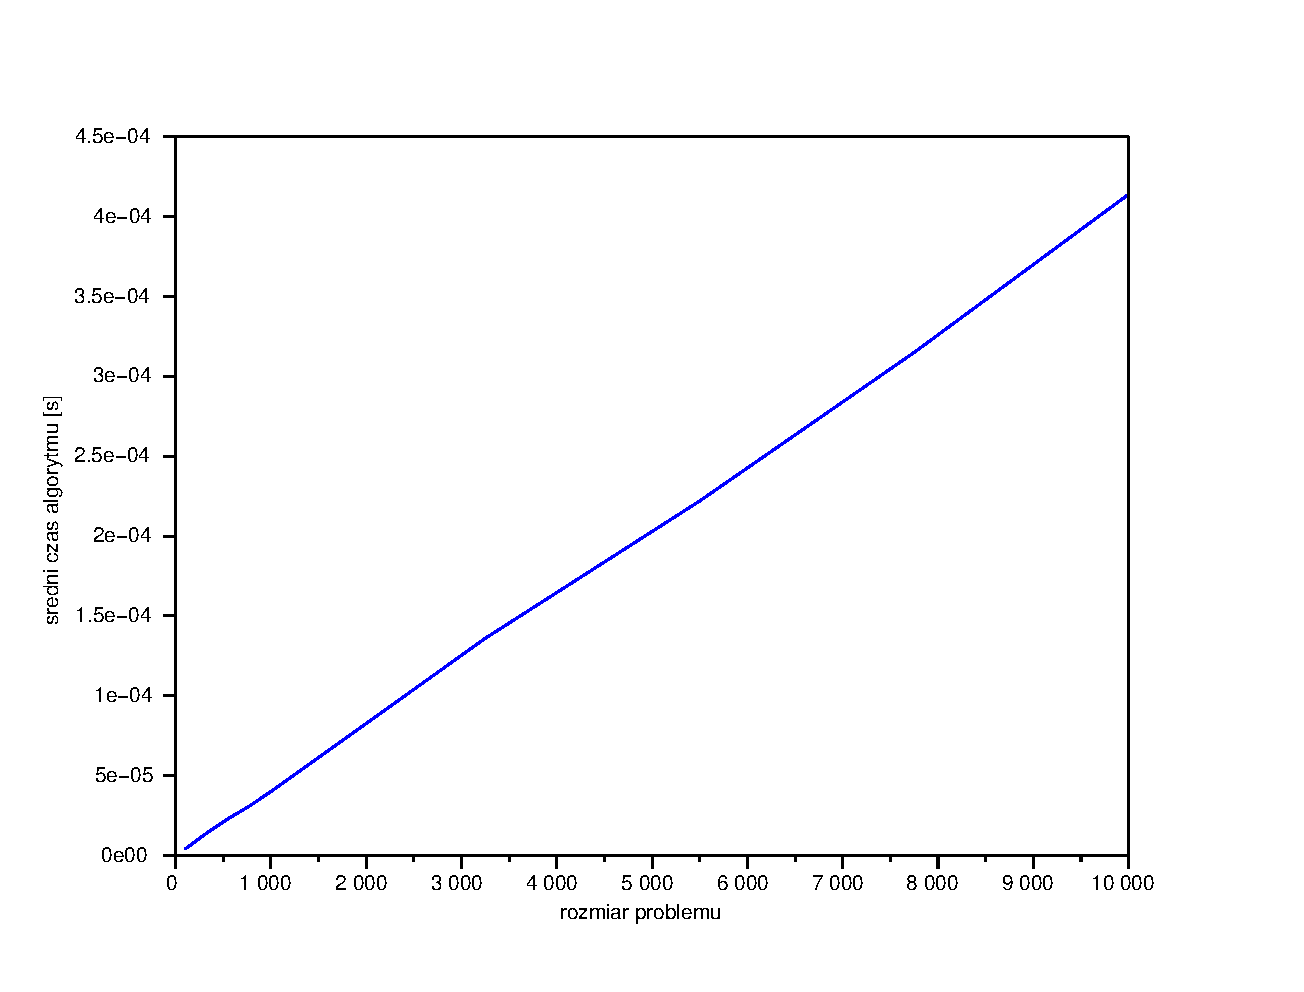
\includegraphics[width=\textwidth]{files/stack.eps}
\caption{Zależność czasu wykonywania algorytmu od rozmiaru problemu dla stosu. \label{stack}} 
\end{figure}

\newpage
\subsection {Stos operujący na tablicach --- wydajniejszy}
Wykonuje podstawowe operacje na stosie. W przypadku przekroczenia rozmiaru tablicy zwiększa jej rozmiar dwukrotnie.

\begin{figure}[!htp]
\centering
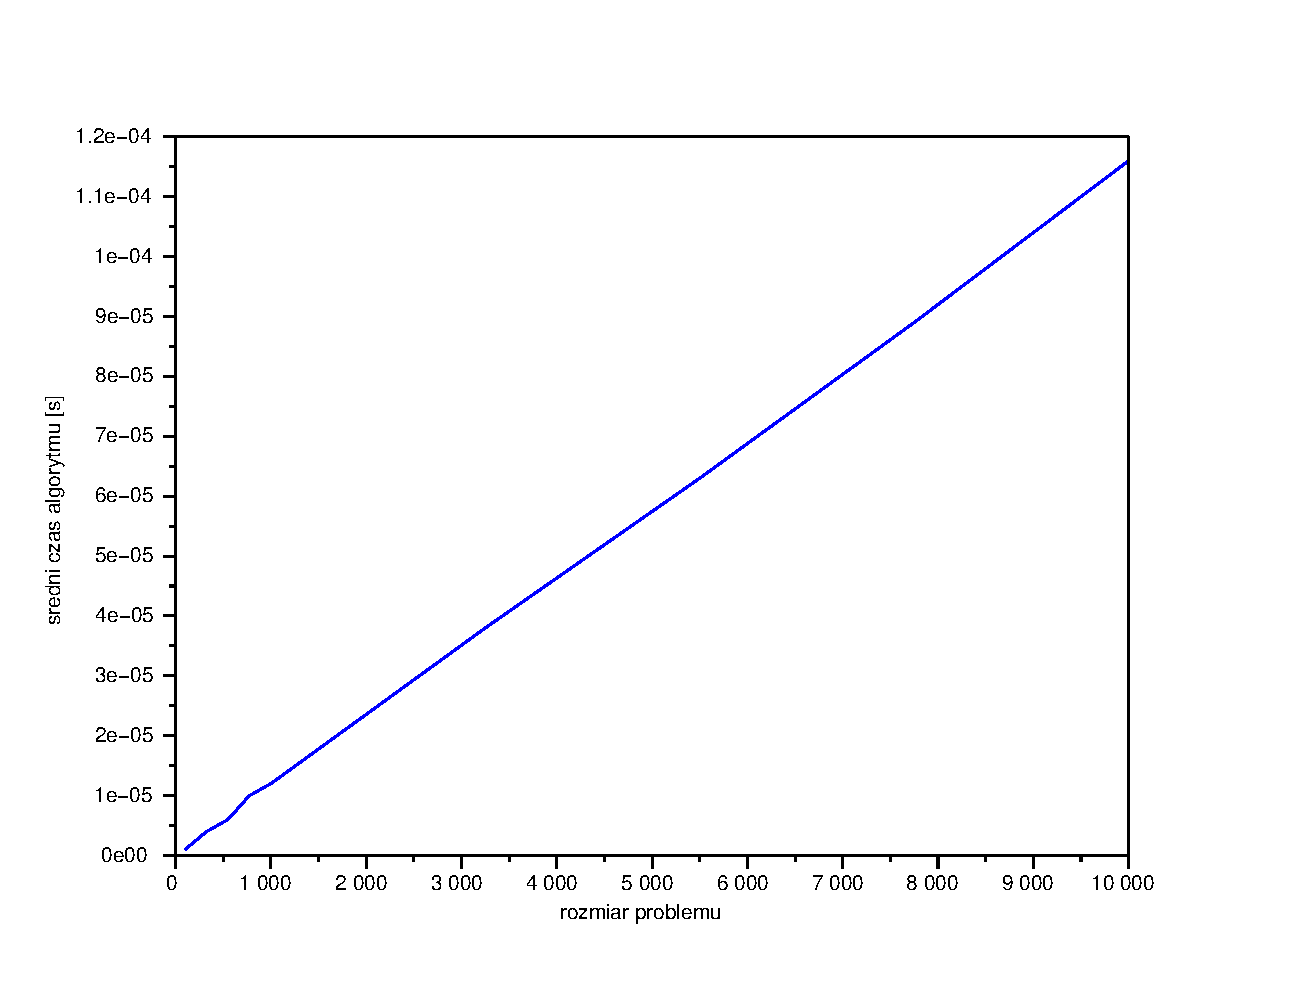
\includegraphics[width=\textwidth]{files/stack2.eps}
\caption{Zależność czasu wykonywania algorytmu od rozmiaru problemu dla stosu --- wersja zoptymalizowana. \label{stack2}} 
\end{figure}

\newpage
\subsection {Stos operujący na liście}
Wykonuje podstawowe operacje stosu na liscie.

\begin{figure}[!htp]
\centering
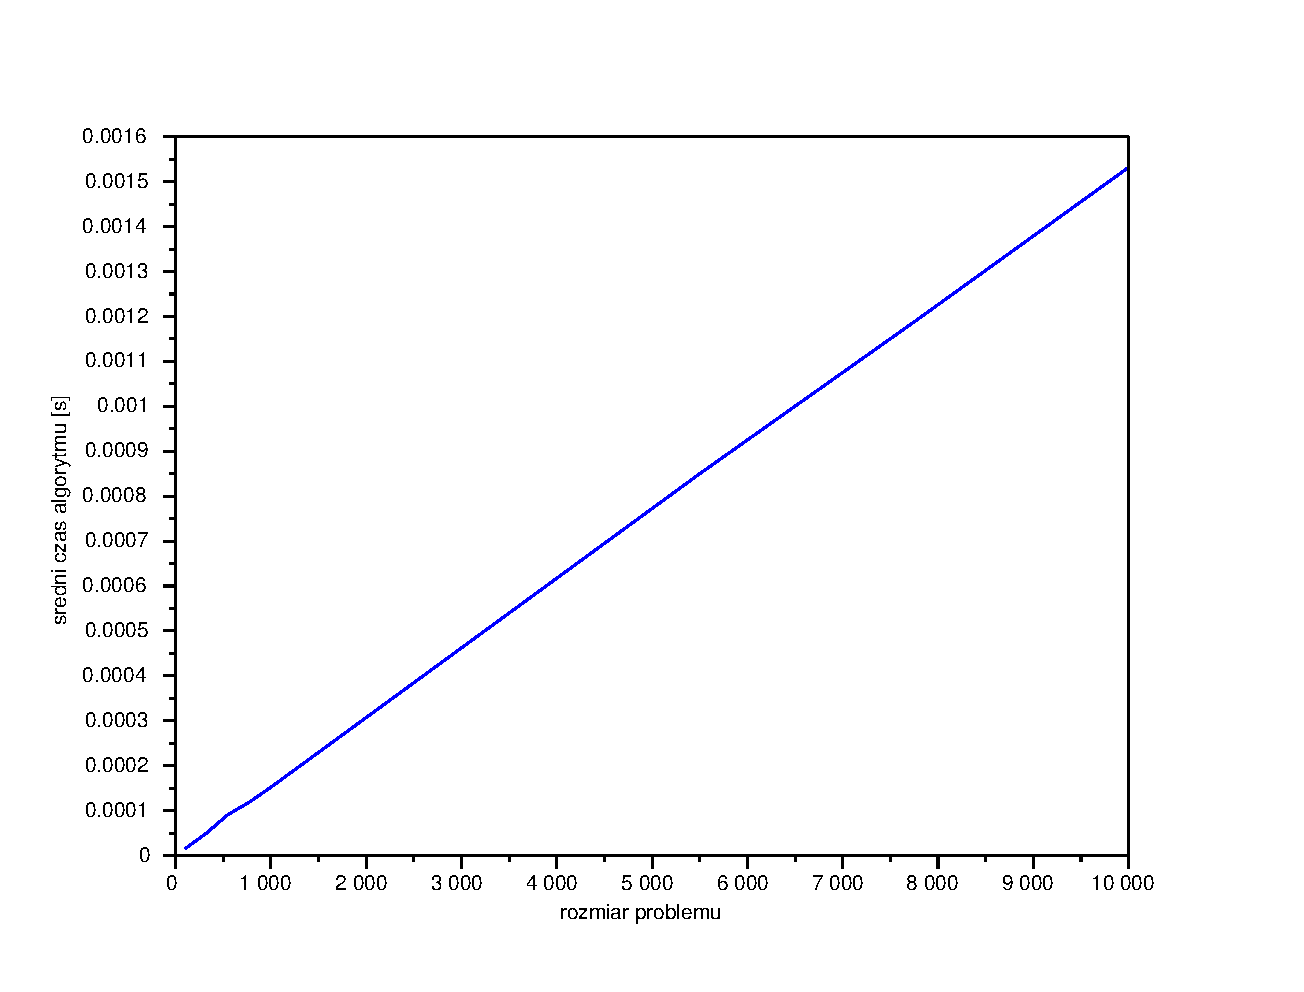
\includegraphics[width=\textwidth]{files/stonlist.eps}
\caption{Zależność czasu wykonywania algorytmu od rozmiaru problemu dla stosu na liście. \label{stonlist}} 
\end{figure}

\newpage
\subsection {Kolejka operująca na liście jednokierunkowej}
Wykonuje podstawowe operacje na kolejce (liście jednokierunkowej).

\begin{figure}[!htp]
\centering
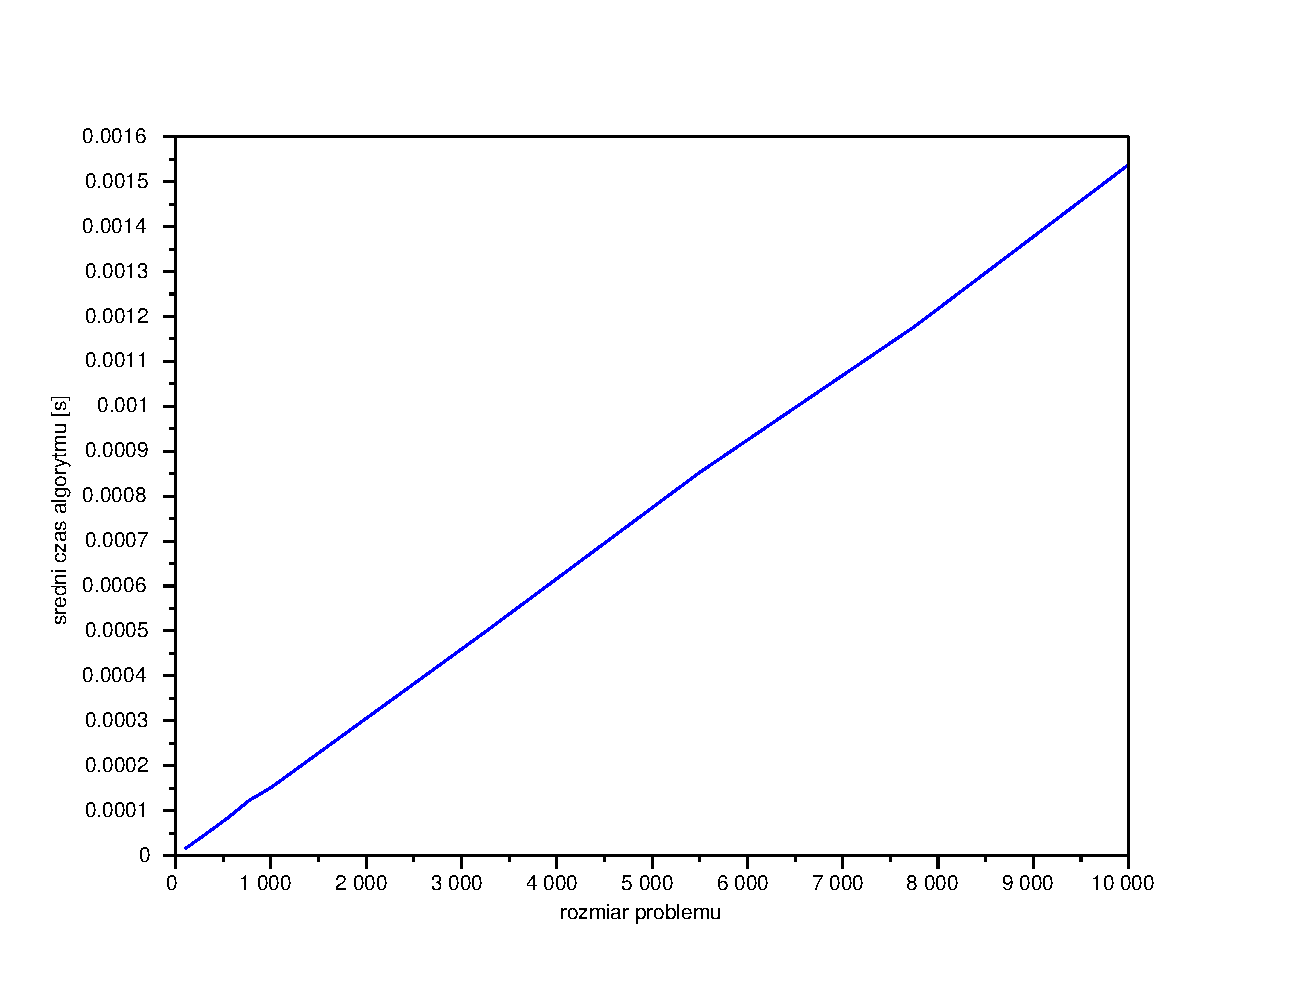
\includegraphics[width=\textwidth]{files/queue.eps}
\caption{Zależność czasu wykonywania algorytmu od rozmiaru problemu dla kolejki. \label{queue}} 
\end{figure}

\newpage
\subsection {Wykres zbiorczy}
Porównanie czasu wykonywania poszczególnych implementacji.

\begin{figure}[!htp]
\centering
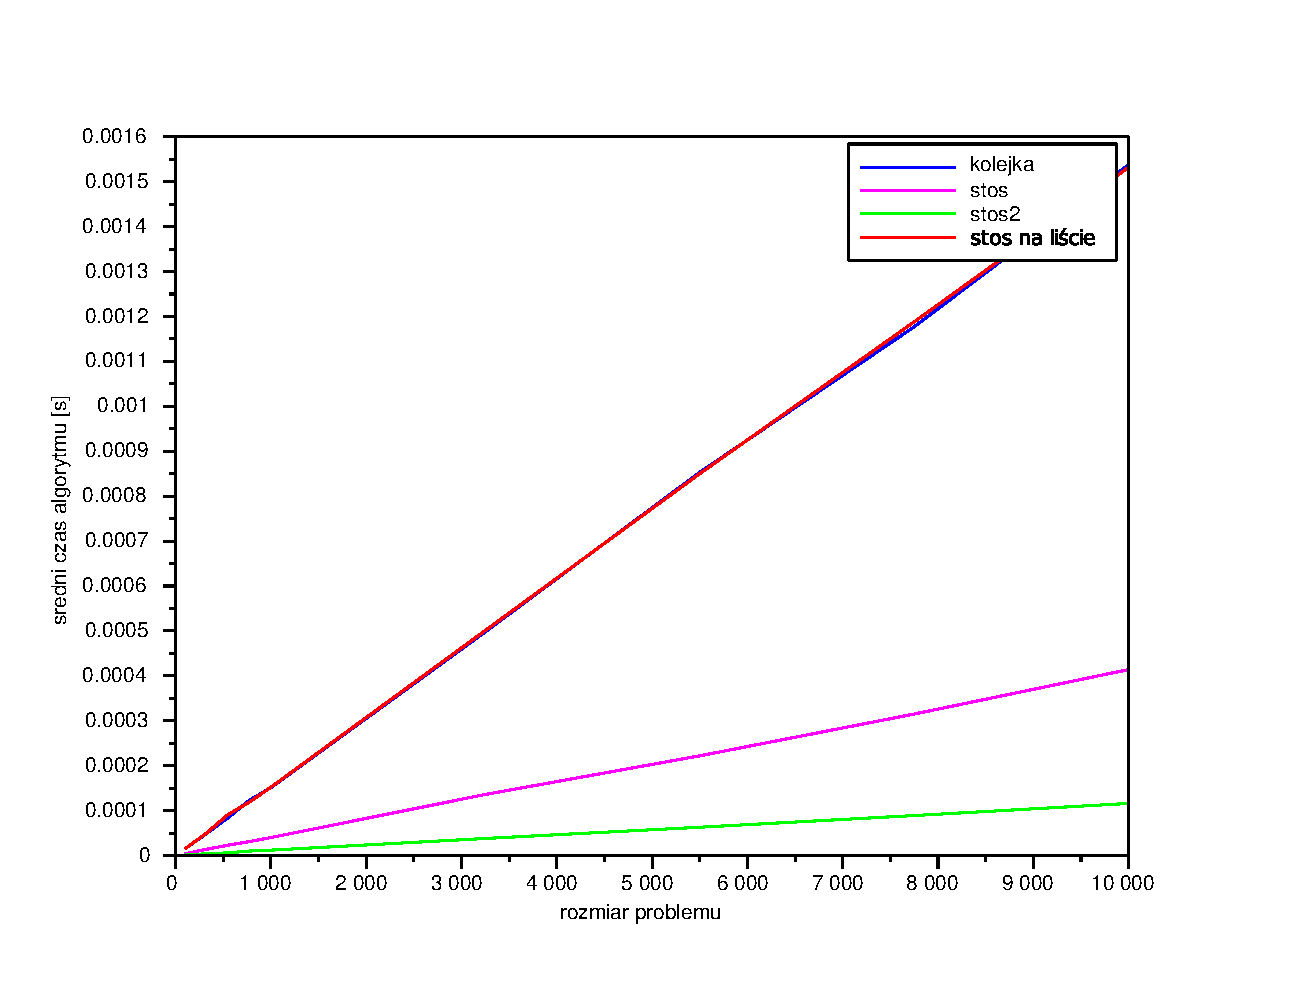
\includegraphics[width=\textwidth]{files/all.eps}
\caption{Zależność czasu wykonywania algorytmu od rozmiaru problemu dla wszystkich implementacji. \label{all}} 
\textit{*\textbf{stos2} - implementacja dla stosu na tablicy --- wersja wydajniejsza}
\end{figure}


\section{Wnioski\label{wnioski}}
\begin{itemize}
\item Wszystkie zależności są w przybliżeniu liniowe. Drobne odkształcenia wynikają z błędów pomiarowych (np.: przez programy pracujące w tle).
\item Najszybszy jest algorytm operujący na tablicy, której rozmiar w przypadku braku miejsca zwiększamy dwukrotnie.
\item Najwolniej działają algorytmy zaimplementowane na listach. W związku z tym lepszym rozwiązaniem jest operowanie na tablicach.
\item Algorytmy kolejki i stosu działają z taką samą szybkością, ponieważ są implementowane w ten sam sposób.
\end{itemize}


\section{Załączniki}
\begin{itemize}
\item Dokumentacja z Doxygena "Dokumentacja.pdf"
\end{itemize}

\section{Dodatkowy wykres, poprawki}
Zwiększając rozmiar problemu przy implementacji tablicy w której po przekoroczeniu rozmiaru zwiększamy go o jeden zależność jest w dalszym ciągu w przybliżeniu liniowa (Rysunek \ref{add}). Jest to zasługa obecnych możliwości sprzętowych (szybkości kopiowania, optymalnym wykorzystaniem poszczególnych funkcji procesora itp.).
\begin{figure}[!htp]
\centering
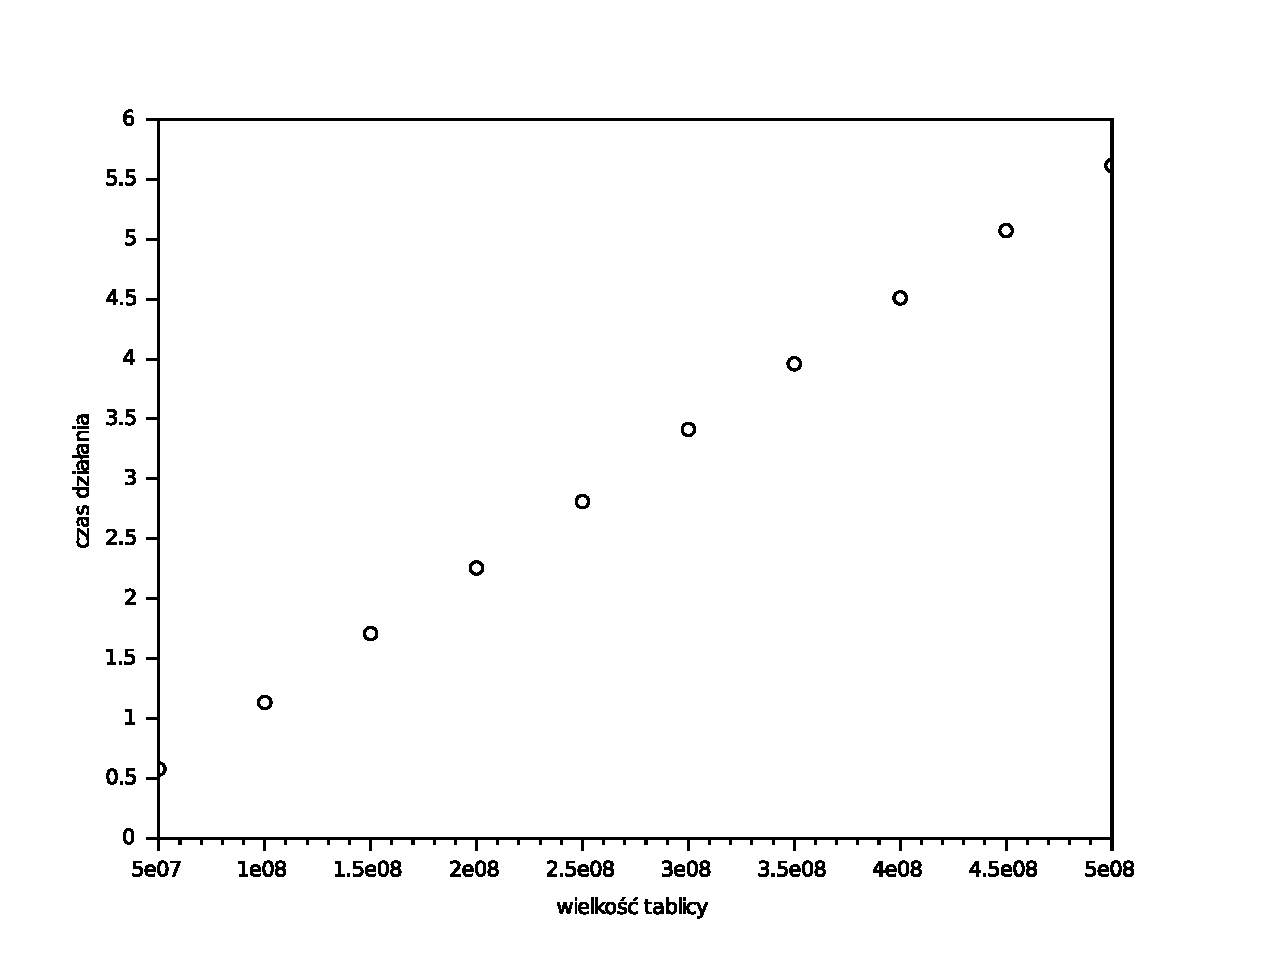
\includegraphics[width=\textwidth]{files/plot.pdf}
\caption{Zależność czasu wykonywania algorytmu od rozmiaru problemu dla tablicy zwiększającej rozmiar o 1. \label{add}} 

\end{figure}

\end{document}
